%
% TCC - César Malerba - Ciência da Computação - INF/UFRGS
%
\documentclass[t]{iiufrgs}
% um tipo especfico de monografia pode ser informado como parmetro opcional:
%\documentclass[tese]{iiufrgs}
% monografias em ingls devem receber o parmetro `english':
%\documentclass[diss,english]{iiufrgs}
% a opo `openright' pode ser usada para forar incios de captulos
% em pginas mpares
% \documentclass[openright]{iiufrgs}
% para gerar uma verso somente-frente, basta utilizar a opo `oneside':
% \documentclass[oneside]{iiufrgs}
\usepackage[T1]{fontenc}        % pacote para conj. de caracteres correto
\usepackage[utf8]{inputenc}   % pacote para acentuação
\usepackage{graphicx}           % pacote para importar figuras
\graphicspath{{./figs/}}
\DeclareGraphicsExtensions{.pdf,.jpg,.png}

\usepackage{times}              % pacote para usar fonte Adobe Times
%\usepackage{mathptmx}          % p/ usar fonte Adobe Times nas frmulas

%
% Informaes gerais
%
\title{Exploits: técnicas, detecção e prevenção}

\author{Malerba}{César}
% alguns documentos podem ter varios autores:
%\author{Flaumann}{Frida Gutenberg}
%\author{Flaumann}{Klaus Gutenberg}

% orientador e co-orientador so opcionais (no diga isso pra eles :))
\advisor[Prof.~Dr.]{Weber}{Raul Fernando}
%\coadvisor[Prof.~Dr.]{Knuth}{Donald Ervin}

% a data deve ser a da defesa; se nao especificada, so gerados
% mes e ano correntes
%\date{maio}{2001}

% o nome do curso pode ser redefinido (ex. para TCs)
\course{Ciência da Computação}

% o local de realizao do trabalho pode ser especificado (ex. para TCs)
% com o comando \location:
\location{Porto Alegre}{RS}

% itens individuais da nominata podem ser redefinidos com os comandos
% abaixo:
% \renewcommand{\nominataReit}{Prof\textsuperscript{a}.~Wrana Maria Panizzi}
% \renewcommand{\nominataReitname}{Reitora}
% \renewcommand{\nominataPRE}{Prof.~Jos{\'e} Carlos Ferraz Hennemann}
% \renewcommand{\nominataPREname}{Pr{\'o}-Reitor de Ensino}
% \renewcommand{\nominataPRAPG}{Prof\textsuperscript{a}.~Joc{\'e}lia Grazia}
% \renewcommand{\nominataPRAPGname}{Pr{\'o}-Reitora Adjunta de P{\'o}s-Gradua{\c{c}}{\~a}o}
% \renewcommand{\nominataDir}{Prof.~Philippe Olivier Alexandre Navaux}
% \renewcommand{\nominataDirname}{Diretor do Instituto de Inform{\'a}tica}
% \renewcommand{\nominataCoord}{Prof.~Carlos Alberto Heuser}
% \renewcommand{\nominataCoordname}{Coordenador do PPGC}
% \renewcommand{\nominataBibchefe}{Beatriz Regina Bastos Haro}
% \renewcommand{\nominataBibchefename}{Bibliotec{\'a}ria-chefe do Instituto de Inform{\'a}tica}
% \renewcommand{\nominataChefeINA}{Prof.~Jos{\'e} Valdeni de Lima}
% \renewcommand{\nominataChefeINAname}{Chefe do \deptINA}
% \renewcommand{\nominataChefeINT}{Prof.~Leila Ribeiro}
% \renewcommand{\nominataChefeINTname}{Chefe do \deptINT}

% A seguir so apresentados comandos especficos para alguns
% tipos de documentos.

% Relatrio de Pesquisa [rp]:
% \rp{123}             % numero do rp
% \financ{CNPq, CAPES} % orgaos financiadores

% Trabalho Individual [ti]:
% \ti{123}     % numero do TI
% \ti[II]{456} % no caso de ser o segundo TI

% Trabalho de Concluso [tc]:
% alm de definir explicitamente o nome do curso (\course) e o local
% de realizao (\location),  necessrio redefinir a nominata,
% pois as informaes necessrias dependem do curso. Ex.:
%\renewcommand{\nominata}{
%        UNIVERSIDADE FEDERAL DO RIO GRANDE DO SUL\\
%        Reitora: Prof\textsuperscript{a}.~Wrana Maria Panizzi\\
%        Pr-Reitor de Ensino: Prof.~Jos Carlos Ferraz Hennemann\\
%        Diretor do Instituto de Informtica: Prof.~Philippe Olivier Alexandre Navaux\\
%        Coordenador do curso: Prof.~Seu Creysson\\
%        Bibliotecria-chefe do Instituto de Informtica: Beatriz Regina Bastos Haro
%}

% Monografias de Especializao [espec]:
% \espec{Redes e Sistemas Distribudos}      % nome do curso
% \coord[Profa.~Dra.]{Weber}{Taisy da Silva} % coordenador do curso
% \dept{INA}                                 % departamento relacionado

%
% palavras-chave
% iniciar todas com letras minsculas, exceto no caso de abreviaturas
%
\keyword{segurança}
\keyword{teste de software}
\keyword{exploits}

%
% inicio do documento
%
\begin{document}

% folha de rosto
% s vezes  necessrio redefinir algum comando logo antes de produzir
% a folha de rosto:
% \renewcommand{\coordname}{Coordenadora do Curso}
\maketitle

% dedicatoria
\clearpage
\begin{flushright}
\mbox{}\vfill
{\sffamily\itshape
``If I have seen farther than others,\\
it is because I stood on the shoulders of giants.''\\}
--- \textsc{Sir~Isaac Newton}
\end{flushright}

% agradecimentois
\chapter*{Agradecimentos}
Estou por agradecer\ldots

% sumario
\tableofcontents

% lista de abreviaturas e siglas
% o parametro deve ser a abreviatura mais longa
\begin{listofabbrv}{SPMD}
        \item[EBP] Extended Base Pointer
		\item[ESP] Extended Stack Pointer
        \item[NUMA] Non-Uniform Memory Access
        \item[SIMD] Single Instruction Multiple Data
        \item[SPMD] Single Program Multiple Data
\end{listofabbrv}

% idem para a lista de smbolos
%\begin{listofsymbols}{$\alpha\beta\pi\omega$}
%       \item[$\sum{\frac{a}{b}}$] Somatrio do produtrio
%       \item[$\alpha\beta\pi\omega$] Fator de inconstncia do resultado
%\end{listofsymbols}

% lista de figuras
\listoffigures

% lista de tabelas
%\listoftables

% resumo na lngua do documento
\begin{abstract}
a escrever\ldots
\end{abstract}

% resumo na outra língua
% como parametros devem ser passados o título e as palavras-chave
% na outra língua, separadas por vírgulas
\begin{englishabstract}{Exploits: técnicas, detecção e prevenção}{security, exploits, testing}
to be written\ldots
\end{englishabstract}

% capítulos em arquivo próprio

\chapter{Conceitos iniciais}
\label{chap:conceitos_iniciais}

	\section{Exploit/Vulnerabilidade}
	O primeiro termo que devemos definir neste trabalho é exploit. Mas antes dele,
	trataremos de vulnerabilidade - pois eles têm uma ligação estreita.
	Podemos definir vulnerabilidade como uma falha em um sistema que permite
	a um atacante usá-lo de uma forma não prevista pelo projetista \cite{Anley2007}.
	Ou seja, uma vulnerabilidade implica a possibilidade de uso indevido de um sistema.
	Os passos necessários para explorar essa fraqueza, ou mesmo o código (programa) que pode tirar
	proveito da vulnerabilidade é descrito como exploit.
	Um exploit surge apenas quando há uma vulnerabilidade - mas podem existir
	vulnerabilidades para as quais não exista exploit.


	\section{Conceitos básicos}
	Neste trabalho iremos tratar de exploits na arquitetura x86 de 32 bits. Trata-se da arquitetura de computadores
	pessoais mais difundida nos dias de hoje. Mas boa parte do estudo realizado pode ser aplicada
	a praticamente qualquer outra arquitetura.

	\section{Gerência de memória}
	O controle da memória é um ponto crítico. Falhas nele acabam resultando em vulnerabilidades 
	gravíssimas. Faremos uma breve abordagem sobre o gerenciamento de memória sobre
	o ponto de vista dos exploits.

	Um primeiro ponto a destacar sobre a memória é um princípio básico que norteia
	quase todas as arquiteturas modernas. Dados e instruções não são diferenciados na memória.
	Ou seja, não há uma separação rígida entre instruções que compõem um programa e os dados
	sobre os quais opera. Essa característica foi herdada da arquitetura básica de von Neumann.
	Como veremos a seguir, essa decisão de design, com origem nos anos 1940, embora tenha
	facilitado a evolução dos computadores, abriu caminhos para os exploits que conhecemos hoje. 

	Abaixo descrevemos o layout básico da memória de um processo em um sistema UNIX.
	Ele pode ser separado em 6 partes fundamentais:
	\begin{description}
		\item[text]
			A parte que contém as instruções do programa - seu código propriamente dito.
			Seu tamanho é fixo durante a execução e ela não deve possibilitar escrita.
		\item[data]
			Contém variáveis globais já inicializadas. Seu tamanho é fixo durante a execução.
		\item[bss]
			Nome de origem história significando Block Started by Symbol. Área da memória responsável
			por armazenar variáveis globais	não inicializadas. Como text e data, bss também tem tamanho 
			fixo conhecido desde o início do processo. 
		\item[Heap]
			Espaço para variáveis alocadas dinamicamente. A chamada de sistema sbrk é responsável
			pelo controle do crescimento/encolhimento desse espaço. Bibliotecas geralmente facilitam a vida
			do programador disponibilizando interfaces mais amigáveis como malloc() e free(). Assim a biblioteca
			se encarrega de chamar sbrk() para diminuir/aumentar o Heap. Ela cresce do endereço mais baixo para o
			mais alto.
		\item[Stack]
			Mantém controle das chamadas de funções. Possibilita a recursividade. Logo, possui
			tamanho variável - crescendo do endereço mais alto para o mais baixo (sendo antagonista do Heap - ver
			figura \ref{fig:regioes_memoria}). 
			Esse crescimento é que torna possível que uma chamada de função que tenha seus dados
			sobrescritos influencie numa chamada de função anterior. Esse é o princípio do buffer overflow - tratado
			posteriormente.
		\item[Enviroment]
			A última porção de memória do processo guarda uma cópia das variáveis de ambiente do sistema.
			Essa seção possui permissão de escrita, mas como bss, data e text, possui tamanho fixo.
	\end{description}

	\begin{figure}
		\begin{center}
		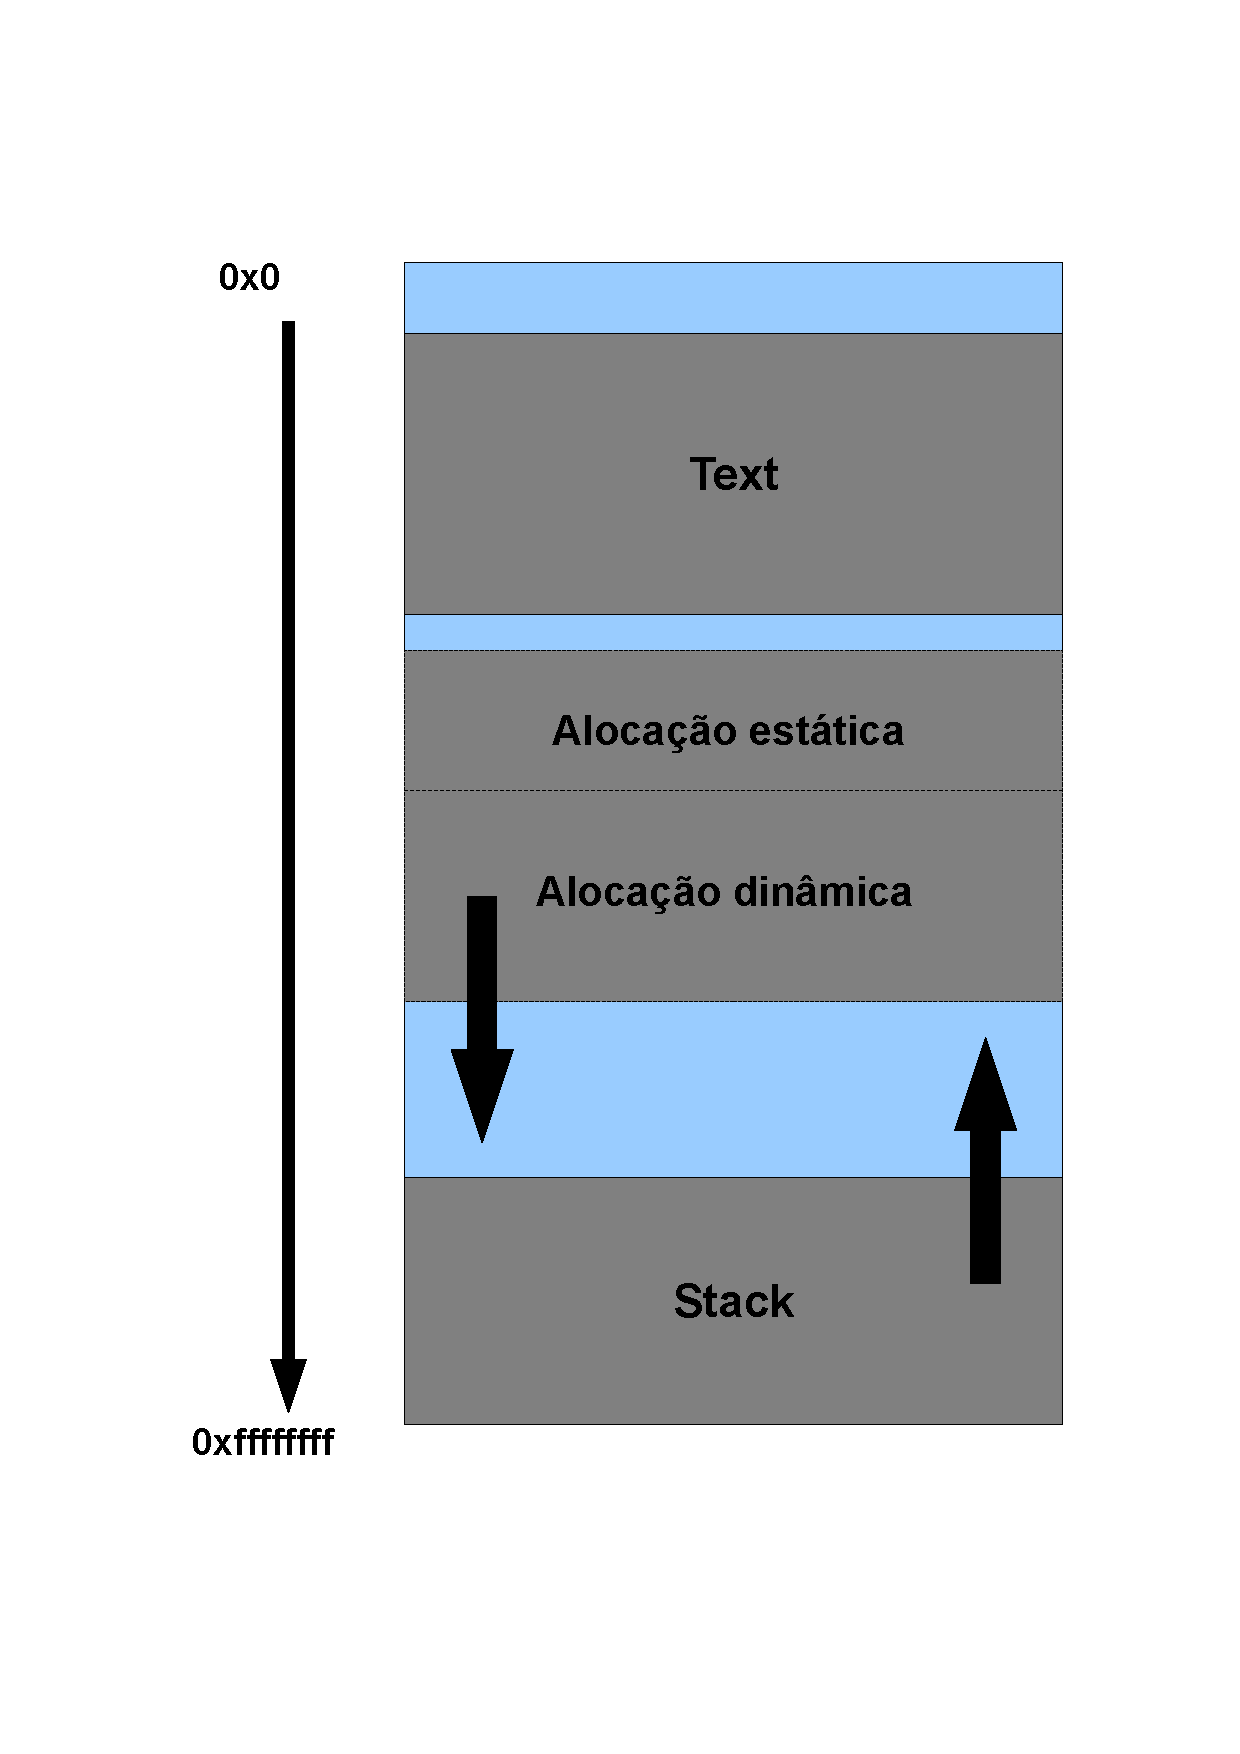
\includegraphics[width=0.45\textwidth]{regioes_memoria.pdf}
		\caption{Regiões de memória em um processo.}
		\label{fig:regioes_memoria}
		\end{center}
	\end{figure}

	\section{Funcionamento mais detalhado do Stack}

	\section{Funcionamento mais detalhado do Heap}
	A porção de memória correspondente ao heap possibilita ao programador alocar dinamicamente memória
	que fica disponível durante toda a execução para qualquer chamada de função. Diferentemente
	da memória alocada no stack - que é perdida quando a função retorna.

	\section{Registradores de controle}
	Uma parte fundamental da arquitetura que deve ser mencionada são os registradores que possuem
	relação direta com o gerenciamento da memória.
	Talvez o mais importante (na arquitetura base do estudo IA32) seja o EIP(Extended Instruction Pointer).
	Ele indica o endereço da próxima instrução. Sobrescrevê-lo equivale obter o controle
	do fluxo de um processo.
	Além dele, destacamos EBP(Extended Base Pointer) e ESP(Extended Stack Pointer).
	ESP indica o endereço do último valor inserido na pilha.
	O EBP indica o início da pilha para aquela chamada de função. É usado para referenciar variáveis
	locais da função.




\chapter{Classificação de vulnerabilidades}
\label{chap:classificacao}

	A classificação de vulnerabilidades representa enorme desafio.
	Nos dias de hoje, não existe nenhum padrão aceito globalmente para essa tarefa.
	Ainda assim, já houve vários avanços na área. 
	Existem padrões para enumerar e catalogar vulnerabilidades, bem como propostas
	que podem criar bases para uma classificação que venha a ser aceita pela comunidade.
	Métricas, relativas	à gravidade e ao impacto, também estão disponíveis
	e são empregadas no auxílio às instituições nas tomadas	de decisões.

	
	No trabalho de Seacord e Householder, \cite{Seacord2005}, temos os fatores que motivam a
	busca pela organização das vulnerabilidades em classes:
	\begin{itemize}
		\item{O entendimento das ameaças que elas representam;}
		\item{Correlacionamento de incidentes, de \textsl{exploits} e de artefatos;}
		\item{Avaliação da efetividade das ações de defesa;}
		\item{Descoberta de tendências de vulnerabilidades;}
	\end{itemize}

	
	Vemos, portanto, que a taxonomia\footnote{Ciência da classificação.} das vulnerabilidades
	pode trazer uma série de benefícios para seu entendimento, tratamento e prevenção.
	Nesse capítulo, nosso intuito é abordar a dificuldade nesse processo e apresentar
	os avanços já obtidos nesse sentido.  


	\section{A dificuldade em classificar; estágio já alcançado: enumeração}
		Antes de entrarmos no mérito das vulnerabilidades, é preciso definir
		com precisão dois termos que utilizaremos por todo o capítulo: classificar e enumerar.
		Como veremos, a taxonomia é mais custosa que a enumeração.

		\subsection{Classificar}
			\label{subsec:classificar}
			Como podemos encontrar em \cite{Holanda1975}, classificar implica "distribuir em classes e/ou grupos
			segundo um sistema". Logo, para a classificação, é preciso haver uma metodologia que possa
			separar os itens em estudo em diferentes grupos. A ciência que estuda esse processo
			é chamada taxonomia. Ela é guiada, conforme \cite{Gregio2005_1}, pelos princípios taxonômicos.
			São eles:
			\begin{description}
				\item[Exclusão mútua]
					Um item não podem ser categorizado simultaneamente em dois grupos.
				\item[Exaustividade]
					Os grupos, unidos, incluem todas as possibilidades.
				\item[Repetibilidade]
					Diferentes pessoas extraindo a mesma característica do objeto devem concordar com
					o valor observado.
				\item[Aceitabilidade]
					Os critérios devem ser lógicos e intuitivos para serem aceitos pela comunidade.
				\item[Utilidade]
					A classificação pode ser utilizada na obtenção de conhecimento na área de pesquisa.
			\end{description}

			
			Vemos que os critérios para a taxonomia são exigentes e pressupõem uma metodologia
			cuidadosamente gerada para atendê-los. 

		\subsection{Enumerar}
			A enumeração é um processo semelhante a 
			"indicar por números; relacionar metodicamente"; como encontramos
			em \cite{Holanda1975}.
			Trata-se, portanto, de algo muito mais simples que a classificação.
			Mesmo sendo mais simples, é extremamente importante pois permite
			que os itens enumerados sejam facilmente apontados e diferenciados entre si.
			
			
			Sem um procedimento de enumeração dos objetos de estudo, adotado de comum acordo,
			não é possível que duas partes se comuniquem sem risco de cometerem enganos. 
			Quem garante que estão tratando exatamente da mesma coisa naquele momento?
			Logo a enumeração é essencial para o devido entendimento sobre os objetos
			de estudo.

		\subsection{Da enumeração à classificação}
			No trabalho de Mann, \cite{Mann1999}, há um excelente paralelo entre a
			questão abordada nesse capítulo e o advento da tabela 
			periódica\footnote{Dispõe sistematicamente os elementos de acordo com suas propriedades permitindo
			uma análise multidimensional.} na Química. 
			A organização dos elementos da forma como conhecemos hoje na tabela periódica
			foi um processo longo que culminou com as ideias de Dimitri Mendeleev.
			Outros químicos que o precederam foram responsáveis pela identificação e
			listagem dos elementos. Isso possibilitou um melhor estudo e uma maior
			troca de informação precisa entre os pesquisadores.


			Segundo Mann, a tabela periódica só pode ser efetivamente criada graças
			aos esforços daqueles que enumeraram os elementos de forma mais simples
			antes de Mendeleev. O trabalho deles permitiu a interoperabilidade
			necessária para o surgimento da tabela periódica.
			Da mesma forma, nos anos antecedentes a 2000, a comunidade que estudava
			e acompanhava as vulnerabilidades estava num patamar semelhante àqueles
			que precederam Mendeleev. Ou seja, sequer havia uma enumeração mais
			amplamente aceita e reconhecida das vulnerabilidades que permitisse
			avanços suficientes para uma taxonomia.

			
			Citamos o ano de 2000 como parâmetro, pois nessa época, 1999, surgiria um projeto
			que se tornaria referência para a criação de uma padronização da enumeração
			de vulnerabilidades. Não seria ainda um evento comparável à criação da
			tabela periódica para Química (pois não trouxe a taxonomia) 
			mas certamente lançaria as bases para
			a interoperabilidade exigida para estudos mais aprofundados na área.
			Estamos falando da criação do 
			CVE(Common Vulnerabilities and Exposures)\footnote{http://cve.mitre.org}\footnote{Na época
			de sua criação era originalmente conhecido por Common Vulnerabilities Enumeration - vide
			\cite{Meunier2006} pg. 9.}
			pelo MITRE. A seção \ref{sec:cve} traz mais detalhes.


			Podemos dizer, portanto, que atualmente, embora não tenhamos uma taxonomia
			amplamente aceita pela comunidade, já foi atingido o estágio de enumeração.
			Projetos como o CVE podem ser considerados como marcos dessa etapa.
			A seguir, iremos abordar em mais detalhes o surgimento e o funcionamento dele.
			Isso nos possibilitará compreender melhor a complexidade da classificação
			das vulnerabilidades bem como irá facilitar o entendimento dos capítulos
			seguintes que abordam \textsl{exploits}.
			

	\section{CVE}
	\label{sec:cve}

		\subsection{Surgimento e objetivos}
			Para deixar mais nítida a dificuldade de interoperabilidade
			das organizações no que se refere a ameaças de segurança na época
			que antecede o CVE, temos a tabela \ref{tab:torre_babel}, extraída de \cite{Martin2001}.
			Ela	mostra como diferentes organizações se referiam à mesma vulnerabilidade
			em 1998. Trata-se de um verdadeira Torre de Babel.

			\begin{table}
				\begin{tabular}{|l|c|c|}
					\hline
						\textbf{Organização} & \textbf{Como se referia à vulnerabilidade}\\
					\hline
						CERT\footnotemark[1] & CA-96.06.cgi\_example\_code\\
					\hline
						Cisco Systems\footnotemark[2] & http - cgi-phf\\
					\hline
						DARPA & 0x00000025 = http PHF attack\\	
					\hline
						IBM ERS & ERS-SVA-E01-1996:002.1\\	
					\hline
						Security Focus\footnotemark[3] & \#629 - phf Remote Command Execution Vulnerability\\	
					\hline
				\end{tabular}
				\footnotetext[1]{site}
				\footnotetext[2]{site}
				\footnotetext[3]{site}
				\caption{Uma vulnerabilidade: diversos nomes e nenhum entendimento}\label{tab:torre_babel}
			\end{table}
			

			O CVE, como dito anteriormente, surge em 1999 e seu maior objetivo, como podemos
			ler em sua FAQ, \cite{CVE2010}, é tornar mais fácil
			o compartilhamento de informações sobre vulnerabilidades utilizando uma enumeração comum.
			Essa enumeração é realizada através da manutenção de uma lista na qual, conforme
			encontramos em \cite{Santos2004}, valem os seguintes princípios:
			\begin{itemize}
				\item{Atribuição de um nome padronizado e único a cada vulnerabilidade.}
				\item{Independência das diferentes perspectivas em que a vulnerabilidade ocorre.}
				\item{Abertura total voltada ao compartilhamento pleno das informações.}
			\end{itemize}


			Segundo a própria organização, vide \cite{CVE2010}, o CVE não possui um objetivo 
			inicial de conter alguma espécie de taxonomia. Essa é considerada uma área de pesquisa
			ainda em desenvolvimento. É esperado que, com o auxílio prestado pela
			catalogação das vulnerabilidades já constitua um importante passo para que
			isso ocorra.

			\begin{figure}
				\begin{center}
					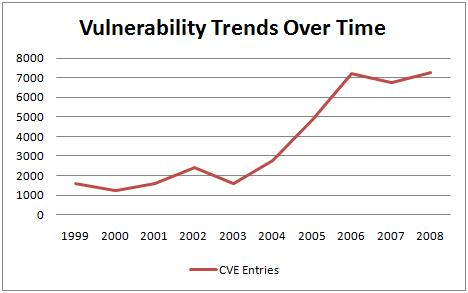
\includegraphics[width=0.65\textwidth]{vulnerabilidades_CVE.jpg}
					\caption{Vulnerabilidades registradas no CVE ao longo do tempo - retirada 
							de \cite{Florian2009}}
					\label{fig:vulnerabilidades_CVE}
				\end{center}
			\end{figure}

			
			Na figura \ref{fig:vulnerabilidades_CVE}, podemos visualizar um histórico
			da quantidade de vulnerabilidades adicionadas. Nos últimos anos podemos
			perceber que os incidentes registrados ficam na média de 7000.
			Isso mostra relevância que o projeto do CVE alcançou.
			
			 
		
		\subsection{Funcionamento}
			O CVE é formado por uma junta de especialistas em segurança dos meios acadêmico, comercial e
			governamental. Eles são responsáveis por analisar e definir o que será feito dos reports passados
			pela comunidade - se eles devem ou não se integrar àqueles já pertencentes à lista.
			Cabe a eles definir nome, descrição e referências para cada nova ameaça.


			Esse processo inicia quando uma vulnerabilidade é reportada.
			Ela assume um CAN(Candidate Number), número de candidata.
			Até que ela seja adicionada à lista, ele permanece com um CAN que
			a identificará. Apenas após o devido estudo e aprovação do caso pela junta
			responsável, é que ela assume um identificador CVE.

			
			Os identificadores CVE são definidos conforme o padrão: CVE-2010-0021.
			Onde, separados por '-', há 3 partes. A primeira é fixa: CVE.
			A segunda refere-se ao ano de surgimento; enquanto a terceira
			indica o número sequencial daquela vulnerabilidade entre todas
			aquelas que foram adicionadas naquele ano. Logo, no exemplo fornecido,
			essa seria a vigésima primeira de 2010.
		
			
			Uma vez integrada, a vulnerabilidade passa a estar publicamente disponível.
			Essa abertura pode servir de auxílio aos atacantes - pois informações
			sobre possíveis furos de segurança são sempre bem vindas a eles.
			Porém, conforme podemos verificar na FAQ do CVE, \cite{CVE2010}, há uma série
			de motivos pelos quais a disponibilidade desses dados supera o risco
			oferecido pela exposição. São eles:
			\begin{itemize}
				\item{O CVE está restrito a publicar vulnerabilidades já conhecidas.}
				\item{Por diversas razões, a comunidade de segurança de informação
					sofre mais para compartilhar dados sobre as ameças
					que os atacantes.}
				\item{É muito mais custo a uma organização proteger toda sua rede
					contra as ameças que a um atacante descobrir e explorar uma delas para
					comprometer alguma das redes.}
			\end{itemize}
			
		
	\section{Propostas taxonômicas}
		\label{sec:prop_taxonomicas}
		Nessa Seção, apresentaremos taxonomias para vulnerabilidades e um projeto, análogo ao CVE,
		que reúne esforços para a padronização da classificação: o CWE.
		Primeiramente, faremos um breve histórico das propostas já criadas com esse fim.
		A seguir, apresentaremos algumas das classificações que consideramos de maior relevância
		e, por fim, trataremos do projeto CWE - que assume importante papel no contexto atual
		na catalogação dos tipos de vulnerabilidades existentes.

		\subsection{Histórico das propostas}
		\label{subsec:historico_prop_taxonomicas}
			Em \cite{Gregio2005}, encontramos um levantamento das 
			dessas alternativas. Mas, como veremos, nenhuma delas atinge os objetivos
			de uma taxonomia plena - apresentados na seção \ref{subsec:classificar}.
			Assim, buscaremos discutir as ideias para as metodologias
			de classificação com o intuito de apontar suas vantagens e fraquezas.

			Em 1976, surge o primeiro estudo, chamado \textsl{Research Into Secure Operating Systems}(RISOS).
			Ele objetivava auxiliar na compreensão das falhas encontradas nos sistemas operacionais
			como MUTICS, GECOS, IBM OS. Foram propostas 7 classes, pág. 328 de \cite{Gregio2005}:
			\begin{itemize}
				\item{Validação incompleta de parâmetros;}
				\item{Validação inconsistente de parâmetros;}
				\item{Compartilhamento implícito de privilégios ou dados confidenciais;}
				\item{Validação assíncrona ou serialização inadequada;}
				\item{Autorização, autenticação ou identificação inadequadas;}
				\item{Violação de proibição de limite;}
				\item{Erro de lógica explorável;}
			\end{itemize}
			Esse estudo teve importância pelo pioneirismo, mas se limitava a problemas
			de sistemas operacionais bem como não atendia a todos os princípios taxonômicos.

	
			Dois anos após o projeto RISOS, em 1978, seria criado o \textsl{Protection Analysis}(PA).
			Seu objetivo principal era permitir que qualquer pessoa, mesmo sem conhecimento
			específico sobre falhas de segurança, utilizando um padrão dirigido, pudesse
			encontrar vulnerabilidades nos sistemas - \cite{Katrina2005}, pág. 2.
			O PA, separava as falhas em 4 grandes classes - \cite{Gregio2005}, pág. 329:
			\begin{itemize}
				\item{Reforço e inicialização do domínio da proteção;}
				\item{Validação de operandos / dependências no gerenciamento das filas;}
				\item{Sincronização imprópria;}
				\item{Erros de seleção de operadores críticos;}
			\end{itemize}
			Embora a ideia inicial do PA também incluísse a detecção automática de vulnerabilidades,
			sendo pioneiro nesse ponto, a classificação proposta não era intuitiva e de difícil aplicação -
			conforme consta em \cite{Katrina2005}. Logo, a aplicação prática não foi levada adiante, mas
			a base da proposta adicionou conhecimento na área.


			Segundo \cite{Gregio2005}, apenas no ano de 1992, teríamos uma nova proposta
			de classificação que trouxesse nova perspectiva ao estudo em questão.
			Trata-se do trabalho de Landwher: \textsl{A Taxonomy of Computer Security Flaws}.
			Seu foco estava no auxílio aos projetistas no desenvolvimento mais seguro do software.
			Sua classificação tinha por base 3 critérios:
			\begin{itemize}
				\item{Como o defeito entra no sistema(gênese);}
				\item{Quando o defeito entrou no sistema(tempo de introdução);}
				\item{Onde ele se manifesta(localização);}
			\end{itemize}
			De acordo com Grégio, seu principal problema era a ambiguidade no processo de classificação.
			A dependência na visão do classificador tem do sistema impede a objetividade necessária
			a uma boa taxonomia.
			Outro problema nessa proposição, abordado por Katrina, em \cite{Katrina2005}, está
			na dificuldade que pode surgir caso, por exemplo, se desconheça a forma como a vulnerabilidade
			adentrou o sistema. Em tal situação, não seria possível identificar a gênese.
			
			
			No ano de 1996, a taxonomia proposta por Aslam, em \textsl{Use of a Taxonomy of Security Faults},
			traria nova acréscimo às pesquisas na área. Segundo, \cite{Katrina2005}(pág. 3), o esquema
			proposto por Aslam é bastante preciso; consistindo numa série de perguntas para cada
			categoria de vulnerabilidade. Em \cite{Gregio2005}(pág. 329), encontramos as 
			classes criadas por Aslam, com suas subdivisões:
			\begin{enumerate}
				\item{Falhas de codificação;}
					\subitem{Erros de sincronização;}
					\subitem{Erros na validação de condição;}
				\item{Falhas emergentes;}
					\subitem{Erros de configuração;}
					\subitem{Falhas no ambiente;}
			\end{enumerate}
			Embora seja uma taxonomia precisa, conforme ressaltado anteriormente, ela sofre
			por estar focada excessivamente em sistemais UNIX - como indicado em \cite{Katrina2005}.
			

		\subsection{Taxonomias e classificações mais recentes}
		\label{subsec:prop_taxonomicas_recentes}
			Agora trataremos das propostas para classificação de vulnerabilidades que surgiram
			mais recentemente (após 2005) e que merecem uma análise mais apurada. São eles:
			\begin{itemize}
				\item{\textsl{Preliminary List of Vulnerability Examples for Researchers}(PLOVER);}
				\item{\textsl{Comprehesive, Lightweight Application Security Process}(CLASP);}
				\item{\textsl{Seven Pernicious Kingdoms};}
			\end{itemize}
			São taxonomias que não passam pelo rigor científico, pois não atendem a todos
			os princípios taxonômicos, mas que ainda assim acrescentam bastante sobre o
			entendimento dos problemas que as vulnerabilidades representam. É o que
			diz Meunier em \cite{Meunier2006} ao tratar das classificações populares.


			O PLOVER, criado em 2005 por Steve Christey, é um esquema de classificação
			que possui dezenas de categorias principais e, naturalmente, possui ainda mais precisão
			do que a proposição de Aslam. Trata-se de um trabalho com sólidas fundações, pois
			apresenta um \textsl{Framework} conceitual que permite discutir as vulnerabilidades
			em diversos níveis. Ele pode ser encontrado em detalhes em \cite{Christey2006}.
			Dentre as suas contribuições, destacam-se o caráter prático; mais de 1400 vulnerabilidades
			identificadas no CVE foram devidamente classificadas utilizando esse sistema.


			Do trabalho de John Viega e outros colaboradores, temos o CLASP. É um conjunto
			de atividades que busca melhorar a segurança dos sistemas.
			As classes mais básicas são:
			\begin{itemize}
				\item{Erros de range e de tipo;}
				\item{Problemas no ambiente;}
				\item{Erros de sincronização e de temporização;}
				\item{Erros de protocolo;}
				\item{Erros de lógica;}
			\end{itemize}
			


			O \textsl{Seven Pernicious Kingdoms}.
		
		\subsection{O projeto CWE}
						

			

	\section{Métricas para vulnerabilidades: CVSS}
		Comparar objetivamente vulnerabilidades de acordo com sua criticidade é
		algo muito útil para as organizações.
		Isso possibilita que os gestores mensurem o grau de urgência com que devem
		ser tratadas as ameaças. Podemos considerar esse procedimento
		como um tipo rudimentar de classificação. Ainda que não seja uma taxonomia,
		assume um papel de destaque por permitir um padrão para distinguir
		vulnerabilidades mais graves das demais.

		\subsection{Surgimento do CVSS}
			Para essa finalidade existe uma alternativa relativamente recente, o CVSS
			(Common Vulnerability Scoring System), criado em 2005. 
			Trata-se de um \textsl{framework} aberto para atribuição de escore a vulnerabilidades.
			Ele oferece as seguintes vantagens, encontradas em \cite{Mell2007} - pg. 3:
			\begin{description}
				\item[Padronização de escore de vulnerabilidades]{Quando uma organização normaliza
				os escores de vulnerabilidades em todas suas plataformas de hardware e software,
				ela pode instituir uma política comum de gerenciamento das ameaças.}
				\item[\textsl{Framework} aberto]{A abertura permite que os usuários tenham
				livre acesso para compreenderem as razões das vulnerabilidades assumirem
				esse ou aquele escore.}
				\item[Priorização de riscos]{Quando o escore ambiental é calculado, a vulnerabilidade
				passa a possuir contexto. De tal forma que o risco real que ela representa
				para a organização possa ser mensurado.}
			\end{description}

			
			A organização responsável pelo CVSS é a 
			\textsl{Forum of Incident Response and Security Teams} (FIRST)\footnote{www.first.org}.
			Além do FIRST, as seguintes organizações também cooperaram para seu surgimento:
			\begin{itemize}	
				\item{CERT/CC}
				\item{Cisco}
				\item{DHS/MITRE}
				\item{eBay}
				\item{IBM Internet Security Systems}
				\item{Microsoft}
				\item{Qualys}
				\item{Symantec}
			\end{itemize}	
			Sua primeira versão data de 2005. Desde 2007, já se encontra na segunda versão;
			tratada em \cite{Mell2007}. Nesse trabalho, abordaremos	apenas a versão atual do CVSS.

		\subsection{As métricas usadas}
		\label{subsec:metricas_cvss}
			Para o cálculo do escore de uma vulnerabilidade, o CVSS, na sua versão 2, possui diversas métricas
			que são divididas em 3 grupos principais. 
			em \cite{Mell2007}\footnote{Termos em inglês traduzidos livremente pelo autor.}:
			\begin{description}
				\item[Métricas básicas]{Representam as características fundamentais da vulnerabilidade
				e são constantes com relação ao tempo e ao ambiente.}
				\item[Métricas temporais]{Mudam com o transcorrer do tempo, mas não são suscetíveis
				a fatores ambientais.}
				\item[Métricas ambientais]{Estão relacionadas unicamente ao ambiente em que a vulnerabilidade
				é analisada. Por isso, são absolutamente dependentes das particularidades de cada caso.}
			\end{description}	
			Na tabela \ref{tab:grupos_cvss}, são mostradas as métricas usadas subdivididas nos seus respectivos
			grupos. 

			\begin{table}
				\begin{tabular}{|c|c|c|}
					\hline
					\multicolumn{3}{|c|}{ \textbf{CVSS} } \\
					\hline
					\textbf{Métricas básicas} & \textbf{Métricas Temporais} & \textbf{Métricas Ambientais} \\
					\hline
					Vetor de acesso & Facilidade de exploração & Dano colateral potencial \\
					Complexidade de acesso & Confiabilidade no \textsl{report} & Abundância de alvos\\
					Necessidade de autenticação & Nível de remediação & Importância da confidencialidade \\
					Impacto na confidencialidade & & Importância da integridade\\
					Impacto na integridade & & Importância da disponibilidade \\
					Impacto na disponibilidade & &  \\
					\hline
				\end{tabular}
				\caption{Métricas CVSS por grupo}\label{tab:grupos_cvss}
			\end{table}
			
			
			A seguir, faremos breve explicação de cada uma das métricas dos três grupos - vide
			tabela \ref{tab:grupos_cvss}.
			Para o grupo \textbf{básico}, existem seis critérios. São eles:
			\begin{description}
				\item[Vetor de acesso]{Diz respeito ao nível de acesso necessário para explorar
					a vulnerabilidade. Pode assumir três valores: 
					\textbf{Local}(exige acesso físico ou uma conta \textsl{shell}), 
					\textbf{Rede adjacente}(é preciso ter acesso à rede local)
					ou \textbf{Rede}(indica a chamada vulnerabilidade \textsl{remota} - pode ser disparada
					de qualquer ponto da Internet).}
				\item[Complexidade de acesso]{Indica a complexidade a ser enfrentada
					pelo atacante para que ele, uma vez que tenha obtido acesso ao sistema alvo,
					possa explorar a vulnerabilidade. Assume um dos valores \textbf{alto, médio ou baixo}.
					A complexidade é considerada alta, por exemplo, se o ataque exige alguma
					técnica de engenharia social mais sofisticada ou se existe uma condição de corrida
					com janela muito exígua que deve ser vencida.}
				\item[Necessidade de autenticação]{Mede a quantidade de vezes que o atacante
					é obrigado a se autenticar durante o ataque - mesmo que seja usada a mesma credencial.
					É um dos valores: \textbf{nenhuma, uma, várias}}.
				\item[Impacto na confidencialidade]{Mede o impacto causado
					na abertura de dados confidenciais gerados pelo ataque.
					Se nenhuma informação, em princípio protegida, é comprometida a medida
					assume valor \textbf{nenhum}. Havendo acesso a alguma informação, é considerado
					\textbf{parcial}. É dito \textbf{completo} caso o atacante tenha total acesso
					de leitura aos dados confidenciais.}
				\item[Impacto na integridade]{Avalia a possibilidade que o atacante
					possui de alterar os dados quando o ataque é bem sucedido.
					Se não é mais possível confiar na integridade dos dados após o ataque,
					pois qualquer arquivo pode ter sido modificado, é considerada \textbf{completa}.
					Não havendo possibilidade de alteração, assume o valor \textbf{nenhuma}.
					É denominada \textbf{parcial} quando apenas parte dos dados
					pode ter sido comprometidos.}
				\item[Impacto na disponibilidade]{Indica o quanto a disponibilidade do sistema
					pode ser afetada pelo ataque. É dita \textbf{completa} caso o sistema
					possa ser totalmente desligado ou inutilizado pelo atacante. Assume o valor
					\textbf{nenhuma} quando não pode haver alteração na disponibilidade e
					\textbf{parcial} se o serviço ainda puder estar disponível mas não plenamente.}
			\end{description}
			

			As métricas do grupo \textbf{temporal} são opcionais. Ou seja, podem ser
			desconsideradas no cálculo do escore conforme a vontade nos analistas.
			Por isso, cada uma delas pode assumir o valor \textbf{não definido} indicando
			que ela não deve participar do escore.
			São 3 os critérios que são suscetíveis a alterações com o passar do tempo:
			\begin{description}
				\item[Facilidade de exploração]{Mede o estado atual das técnicas
					e do código disponível para exploração da vulnerabilidade.
					Seus valores são, em ordem crescente de facilidade: 
					\textbf{não comprovada},  \textbf{prova de conceito},
					\textbf{funcional} e \textbf{alta}.
					O primeiro indica que um \textsl{exploit} é meramente teórico
					e não há código disponível que comprove como explorar a falha.
					Havendo código facilmente acessível de \textsl{exploit}
					ou mesmo se operações manuais são suficientes, estamos
					diante de alta facilidade de exploração.}
				\item[Confiabilidade no \textsl{report}]{
					Mede o grau de confiança na existência da vulnerabilidade
					bem como a credibilidade dos detalhes técnicos fornecidos
					quando ela foi reportada. Seus possíveis valores são:
					\textbf{não confirmada}(quando há apenas um rumor de uma origem
					sem credibilidade), \textbf{não corroborada}(há fontes não oficiais
					com possíveis incoerência em seus \textsl{reports}) e \textbf{confirmada}(
					o autor ou o fabricante admitem o problema ou ele já é amplamente
					conhecido existindo até \textsl{exploits} facilmente encontrados).
					}
				\item[Nível de remediação]{Determina o quão longe se está de uma medida
					definitiva para estancamento da vulnerabilidade.
					Logo que o problema surge, assume o valor \textbf{indisponível}.
					Se houver alguma forma, não oficial, de mitigar a vulnerabilidade,
					é dito que a remediação está no estágio de 	\textbf{\textsl{workaround}}.
					Se existe alguma medida oficial, mas ainda não definitiva, 
					seu valor é \textbf{conserto temporário}. O nível é máximo,
					portanto assumindo o escore mínimo,
					\textbf{conserto definitivo}, caso exista uma remediação de caráter
					oficial definitiva.}
			\end{description}



			Os fatores relativos à influência do ambiente, são medidos na \textbf{métricas
			ambientais}. Cada organização pode sofrer diferentemente o impacto de uma
			vulnerabilidade dada a heterogeneidade com que podem se organizar em termos
			do software e hardware utilizados para desempenhar suas funções.
			Exemplificando, caso uma empresa preste algum tipo de serviço de \textsl{backup} de
			dados, a integridade e a confidencialidade da informação que ela mantém
			possuem importância máxima. Em contrapartida, se a atividade desempenhada pela
			empresa estiver relacionada à hospedagem de projetos de código fonte aberto,
			a disponibilidade assume muito maior importância que a confidencialidade.
			Da mesma forma como os critérios temporais, eles podem assumir o valor não definido;
			indicando que ele não é utilizado no cálculo do escore final.
			Abaixo, são explicados os 5 critérios que compõem a métrica temporal:
			\begin{description}
				\item[Dano colateral potencial]{
					Mede o potencial do estrago que a vulnerabilidade pode causar à organização.
					Podem ser danos patrimoniais, pessoais ou relativos a ganhos financeiros.
					Assume os valores(do menor para o maior dano potencial):
					\textbf{nenhum}, \textbf{baixo}, \textbf{baixo-médio}, \textbf{médio-alto} e
					\textbf{alto}}.
				\item[Abundância de alvos]{Mensura a proporção dos possíveis alvos
					sobre o contingente de sistemas da organização.
					Pode ser \textbf{nenhuma}, \textbf{baixa}(1 a 25\%), 
					\textbf{média}(26 a 75\%) e \textbf{alta}(76 a 100\%)
					.}
				\item[Importância da confidencialidade]{Indica a relevância da
					confidencialidade dos dados mantidos pela empresa. Assume os valores
					\textbf{baixo}, \textbf{médio} e \textbf{alto}.}
				\item[Importância da integridade]{Análogo à importância da confidencialidade.}
				\item[Importância da disponibilidade]{Análogo à importância da confidencialidade.}
			\end{description}
		

		\subsection{Cálculo do escore}
			Tendo sido apresentadas as métricas, faremos breve explicação
			do funcionamento do cálculo do escore,
			que varia de 0 a 10, para uma vulnerabilidade.
			A figura \ref{fig:cvss_metricas_equacoes} apresenta uma visão geral desse processo. 
			\begin{figure}
				\begin{center}
					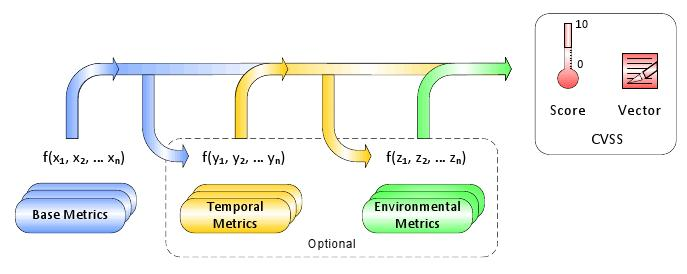
\includegraphics[width=0.85\textwidth]{cvss_metricas_equacoes.jpg}
					\caption{Aplicação das métricas e equações do CVSS - Fonte: \cite{Mell2007}}
					\label{fig:cvss_metricas_equacoes}
				\end{center}
			\end{figure}
			Passos necessários:
			\begin{enumerate}
				\item{Para cada um dos critérios descritos na Seção \ref{subsec:metricas_cvss},
					atribuir um valor válido.}
				\item{Consultar as tabelas, no capítulo	\ref{chap:equacoes_cvss},
					para definir um valor numérico a partir do valor nominal escolhido no passo anterior.}
				\item{Fazer o cálculo do escore básico usando a equação básica disponível em TODO.}
				\item{Fazer o cálculo do escore temporal usando sua respectiva equação TODO,
					 e o escore básico.	Passo opcional. É possível manter apenas o escore básico como o final.}
				\item{Calcular o do escore final usando a equação ambiental, TODO,
					 a partir do escore temporal. Também é opcional; pois os critérios 
					ambientais podem ser desconsiderados.}
			\end{enumerate}
			
			
			Ao final do cálculo, a vulnerabilidade recebe um escore de 0 a 10.
			Sendo 10 o valor da mais crítica possível. É importante destacar, que a atribuição
			dos valores, feita no passo 1, deve ser realizada por especialistas na área seguindo
			um critérios padronizados.

			


\chapter{NULL pointer Exploit}
\label{chap:null_pointer_exploit}

	Dentre as várias técnicas de exploits existentes, uma que certamente merece
	destaque, é o NULL pointer exploit.
	Sua disseminação é recente, sendo fruto da crescente dificuldade em aplicar técnicas
	que exploram vulnerabilidades de corrupção de memória.
	

	Um marco para esse tipo de exploit certamente foi o artigo de Mark Dowd \cite{Dowd2008}.
	A forma como ele trouxe à luz uma falha na máquina virtual do ActionScript chamou
	a atenção de diversos especialistas na área. 
	Isso porque, para muitos, o NULL pointer era apenas sinônimo de um \textsl{bug}
	que resultaria, no máximo, em uma negação de serviço.
	Por isso, o raciocínio empregado por ele serviria de base para encontrar muitos outros problemas.

	
	O ano de 2009 chegou a ser considerado o ano do "kernel NULL pointer deference"
	em virtude da grande quantidade de falhas desse gênero encontradas no kernel do Linux.
	(citar http://cwe.mitre.org/top25/ para o ano de 2009)
	Vemos então que essa falha chegou a atingir notoriedade pelo grande impacto que causou.

	
	Nesse capítulo, nossa intenção é apresentar esse tipo de vulnerabilidade e seu
	correspondente exploit. Assim como identificar os meios de detecção e prevenção. 
	
	
	\section{O que é um NULL pointer}
		O primeiro ponto a ser abordado é o NULL pointer.
		Na linguagem de programação C, podemos considerar um ponteiro como um valor inteiro
		que referencia uma posição de memória. Ou seja, trata-se de um valor que aponta
		para o início de uma determinada região de memória. Quando um ponteiro é deferenciado,
		passamos a acessar o valor presente na posição de memória para o qual ele aponta.
		Ilustrando, segue pequeno trecho de código C.
		\begin{lstlisting}[label=pointer_example,caption=Ponteiro em C]
int val = 10;
int *pointer = &val;
/* pointer has the address of val */

int x = *pointer;
/* *pointer returns 10 */
		\end{lstlisting}
		

		No Linux, o arquivo stddef.h contém a definição de NULL, que por
		convenção, denomina um ponteiro com valor zero.
		Um ponteiro nulo, então, aponta para a posição zero de memória. 
		Como, em regra geral, os sistemas utilizam o esquema de memóra virtual,
		na prática, esse endereço zero deve ser considerado tão somente no espaço
		de endereçamento do processo em questão.
		Como normalmente ele não constitui um mapeamento válido, pois os processos não
		iniciam com aquela porção mapeada, os acessos a essa região implicam violação
		às regras do esquema de memória virtual. Erros como esse resultam
		no término da aplicação. Por isso, na maioria dos casos, um acesso a um ponteiro
		nulo é apenas sinônimo de uma DoS (negação de serviço).


				
		Diversas falhas em uma aplicação real podem levar à presença de um ponteiro zerado.
		Falhas ao inicializar uma estrutura de dados pode deixar ponteiros nulos inadvertidamente.
		Outro possível problema pode ocorrer quando o sistema tem sua memória esgotada e, 
		a chamada responsável por alocar mais espaço retorna NULL, mas como essa possibilidade não é considerada
		pelo programador, o ponteiro a receber esse bloco de memória acaba ficando zerado e a aplicação
		segue normalmente.
		
		Vemos, portanto, que um ponteiro nulo é um caso particular no qual a região de memória
		referenciada é aquela que inicia no endereço zero (no contexto de endereçamento do
		processo em questão - considerado o uso de memória virtual). 
		Exceto em casos especiais, essa situação leva a erros na aplicação que resultam em seu término.
		Conforme trataremos a seguir, há casos em que um ponteiro nulo irá possibilitar um ataque.		

	\section{Como funciona a técnica}
		A técnica de exploração desse tipo de vulnerabilidade irá variar conforme o contexto
		em que surge e como é utilizado o ponteiro nulo. 
		Conforme exposto anteriormente, esse método não é tão genérico como as falhas de \textsl{buffer overflow}.
		São ataques mais focados que exigem ajustes muito maiores em função das especifidades da aplicação alvo.
		Como em outros gêneros de exploits, o objetivo desejado é a escrita de dados fornecidos 
		pelo usuário em endereços arbitrários. Pois isso possibilita, por exemplo,
		a cópia de um \textsl{shellcode} para ser executado. Mas isso não é uma regra, há falhas
		de NULL pointer que envolvem ponteiros para funções que possuem um caminho mais simples
		para exploração.

	
		Para fins de simplificação, vamos dividir os tipos de ataques com essa técnica em duas famílias.
		Como podem existir várias formas de exploração de aplicações em que surgem ponteiros nulos,
		para facilitar a compreensão, vamos tomar dois tipos representativos que são capazes de passar
		a ideia fundamental.
		Numa delas, um endereço que define a localização de uma escrita depende de um ponteiro zerado.
		Em outra, esse ponteiro define uma função a ser executada.
		A primeira chamaremos de \textbf{ponteiro nulo de escrita} e a segunda de \textbf{ponteiro nulo de função}.


		\subsection{Ponteiro nulo de escrita}
		\label{subsec:ponteiro_escrita}
			Nessa situação, por algum motivo, um ponteiro que define um endereço de escrita fica nulo.
			Seja porque a memória alocada foi retornada em NULL e não foi verificada ou mesmo porque
			a aplicação não validou corretamente a entrada e o calculou indevidamente.
			O artigo de Mark Dowd, \cite{Dowd2008}, trata com riqueza de detalhes esse gênero de falha.
			

			Para que uma falha de NULL pointer desse tipo possa resultar em um ataque,
			podemos elencar dois pré-requisitos:
			\begin{itemize}
				\item{O ponteiro nulo é utilizado para calcular o endereço de uma escrita}
				\item{A escrita depende de algo fornecido pelo usuário além do NULL pointer}
				\item{Os dados a serem gravados podem ser controlados de alguma forma pelo usuário}
			\end{itemize}
			Abaixo, ilustrando o que foi exposto, um pequeno trecho de código em linguagem C.
			Nele, o usuário fornece dados, mas como o endereço base de destino de uma cópia está zerado,
			é possível influenciar diretamente na escolha de onde são gravados.
			Essa vulnerabilidade implica a condição do atacante de gravar em um endereço arbitrário dados
			que ele pode controlar - que pode ser um \textsl{shellcode}.
			\begin{lstlisting}[label=write_to_address,caption=Ponteiro em C]
/* user input at user_data */
write_address = null_pointer + offset_influenced_by_user;
/* the address has been 'chosen' by the user */

memcpy(write_address, user_data, certain_size);
/* data is copied from one point to another according to user's will */
			\end{lstlisting}
			
			
		\subsection{Ponteiro nulo de função}
			Ocorre quando, por necessidade de dinamismo, uma função que deve cumprir determinado
			papel, é definida por um ponteiro. Normalmente, ele deve conter um valor válido
			de um endereço de memória que contenha código que cumpra com as ações desejadas.
			Mas isso pode, na prática, não se confirmar. Um valor NULL pode estar no ponteiro
			no momento em que a função é chamada.

			
			Se o endereço zero não constituir uma região válida, a aplicação terminará com um erro.
			Mas e, se pusermos algo nessa região para ser executado? Imagine que um atacante tenha
			posto um \textsl{shellcode} justamente nesse ponto e provocou a chamada função definida pelo
			ponteiro nulo. Aí, certamente, poderíamos estar frente a um ataque com grandes chances de
			ser bem sucedido.
			

			Como pré-requisitos, podemos elencar, portanto:
			\begin{itemize}
				\item{Um ponteiro nulo define o endereço de uma função a ser chamada}
				\item{O usuário pode provocar a chamada dessa função}
				\item{É possível mapear para o endereço zero uma região válida de memória contendo dados do usuário}
			\end{itemize}
			Com esses pontos básicos atendidos, há condições para o emprego da técnica.
			Como exemplo maior, mostraremos um bug no Kernel do Linux na seção \ref{sec:exemplos_null_pointer}. 


	\section{Exemplos reais de NULL pointer exploit}
	\label{sec:exemplos_null_pointer}

		Nessa seção, apresentamos vulnerabilidades reais que exemplificam o exploit em estudo.
		Aquele que não poderia faltar, sem dúvida, é a falha tratada por Mark Dowd pelo fato
		ter servido de inspiração


		Também não poderíamos deixar de analisar os erros encontrados no Kernel do Linux em 2009.
		Isso porque 
			

		\subsection{Falha na máquina virtual do ActionScript}
			Trata-se de uma vulnerabilidade que se enquadra no que denominamos \textbf{ponteiro nulo de escrita} (em 
			\ref{subsec:ponteiro_escrita}).
			Consta no CVE como CVE-2007-0071. Foi objeto do estudo do artigo \cite{Dowd2008}.
			A falha ocorre na leitura de arquivos SWF(Shockwave Flash). Dados no arquivo são usados
			como parâmetros de alocação de memória. Se for passado um valor muito alto, como 2 gigabytes,
			a alocação não é bem sucedida e, por consequência, um ponteiro nulo é retornado.
			A aplicação realiza uma escrita na memória usando como parâmetros do cálculo do endereço de destino
			o ponteiro nulo com outro valor lido do arquivo (escolhido pelo usuário).
			Na página 7 de \cite{Dowd2008}, temos uma versão alto nível desse trecho de código
			em que ocorre o cálculo do endereço de destino e a escrita na memória.
			

			TODO: registrar versões vulneráveis.
			

			O destino da escrita é escolhido pelo usuário quase de forma arbitrária. Existem algumas restrições
			como divisibilidade por 12 quando somado a 4. Mas isso não impede que um ataque seja realizado.
			Como é possível acompanhar em \cite{Dowd2008}, criando um arquivo do tipo SWF da forma
			correta e manipulando detalhes da máquina virtual do ActionScript, o atacante torna-se
			capaz de executar seu \textsl{shellcode} na máquina alvo. Isso é feito através da construção
			de \textsl{bytecode} nativo para a máquina virtual ActionScript que permite a injeção do \textsl{shellcode}.
			Após a execução do último, a aplicação retorna normalmente ao seu fluxo criando a impressão que
			nada demais ocorreu.

			
			Pela enorme base de usuários que utilizam o Flash Player afetado, podemos dizer
			que o impacto da exploração dessa vulnerabilidade foi enorme.
			Principalmente porque a esmagadora maioria dos usuários jamais consideraria um
			uma apresentação em Flash como um potencial vetor de ataque.

			
			Vários fatores foram necessários para que um exploit fosse possível nesse caso.
			Falhas na validação de dados fornecidos pelo usuário foram os mais graves.
			Mas não foram os únicos. A aplicação também não soube lidar corretamente com erros
			na alocação de memória. Essa vulnerabilidade, como tantas outras, portanto, surge
			apenas pela combinação de uma série de problemas que são devidamente concatenados
			por uma mente criativa e obstinada de um atacante.
						
		
		\subsection{Falhas no kernel do Linux}
		\label{subsec:linux_kernel_vuln}
			Existem diversas falhas documentadas no kernel do Linux relacionadas a NULL pointer.
			Desde problemas na inicialização de estruturas de dados até a erros na compilação.		
			Para exemplificar, trataremos de um erro conhecido no CVE como CVE-2009-2692.
			Trata-se de uma vulnerabilidade muito grave que possibilita uma escalada de privilégios
			no sistema.
			
			
			A origem do problema encontra-se na inicialização incorreta de ponteiros de funções em estruturas
			de dados do Kernel (como \textsl{proto\_ops\_structures}). 
			Um \textsl{bug} em uma macro (SOCKOPS\_WRAP) acabava deixando não inicializado
			funções responsáveis, por exemplo, de assumir o controle quando uma operação não disponível fosse
			requisitada. Enquadra-se, portanto, no que convencionamos como \textbf{ponteiro nulo de função}.

			
			Mais especificamente, quando um socket fosse usado e, fosse chamada a função sock\_sendpage,
			e não fosse possível enviar a página, a função sock\_no\_sendpage deveria ser despertada
			para tratar a situação. Mas, conforme explicamos, o valor NULL(zero) estaria ocupando o devido
			local do endereço da função sock\_no\_sendpage. Logo, o contexto da execução seria transferido
			para a região de memória iniciada em zero. Por isso, sendo injetado um código nesse bloco,
			ele seria executado com os privilégios do Kernel.
			TODO: citar http://blog.cr0.org/2009/08/linux-null-pointer-dereference-due-to.html.

	
			A seguir, segue o código que tira proveito dessa vulnerabilidade e possibilita ao atacante
			a execução de código com privilégio máximo no sistema.  
			\lstinputlisting[caption=Exploit para CVE2009-2692]{exemplos_de_codigo_fonte/linux_cve_2009_2692.c}

			
			Essa vulnerabilidade, que podemos considerar de alto impacto mas de simples exploração,
			na nossa avaliação, surge devido a duas falhas gravíssimas.
			A primeira, duramente criticada por especialistas, é o compartilhamento do espaço de endereçamento
			do Kernel do Linux com o processo do usuário. Essa decisão arquitetural
			tornou possível que uma simples chamada a mmap, no processo do usuário, tivesse o alcance de
			mapear a região de memória zero no contexto do Kernel. 
		

		\subsection{NULL pointer em ARM e XScale}
		\label{subsec:null_pointer_arm_xscale}
			Embora o foco do presente trabalho recaia sobre a arquitetura x86, é válido 
			identificar a repercussão de um acesso a posição zero de memória em outros casos.
			Existem arquiteturas nas quais esse endereço já é mapeado inicialmente. 
			Podemos apontar o caso da ARM e da XScale; ambas para sistemas embarcados. 
			Nelas, o vetor de exceções se encontra nessa posição. Ele contém, por exemplo,
			o endereço que define o vetor para o tratamento das interrupções de software.


			Essa vulnerabilidade, é tratada por Barnaby Jack, pesquisador de segurança da Juniper,
			em \cite{Jack2007}. Conforme Jack, caso alguma aplicação nas arquiteturas em questão
			possua alguma falha na qual o endereço de destino de uma escrita seja um ponteiro nulo,
			o vetor de exceções acaba sendo sobrescrito. Isso potencializa enormemente um erro
			de NULL pointer.


			Como exemplo, em \cite{Jack2007}, é apresentada uma falha na biblioteca libpng.
			Um tratamento inadequado da alocação de memória para imagens, que
			retornava NULL, permitia que os dados de uma imagem fossem copiados
			via memcpy() para o endereço zero. Por esse caminho, um atacante seria capaz
			de sobrescrever a tabela de endereços de interrupções de software.
			Assim, bastaria uma chamada do sistema em virtude de uma interrupção,
			para que o código injetado pudesse ser executado.

			
			Segundo avaliação de Jack, uma das formas de prevenir esse tipo de ataque é
			não permitir a escrita na área do vetor de exceções. Outra medida sugerida,
			e existente em versões posteriores das arquiteturas, como ARM9, é a possibilidade
			de mapeamento do vetor de exceções para endereços mais altos - como 0xFFFF00000.
			De qualquer forma, não resta dúvida que os projetistas cometeram sério
			equívoco nas escolhas envolvidas no vetor de exceções.
				
						

	\section{Como evitar o problema}
		Há vários caminhos que podem convergir para que não existam vulnerabilidades causadas 
		por ponteiros nulos. Nas seções anteriores, foram abordados diversos aspectos que
		demonstraram porque o problema existe e os pré-requisitos para que ele seja explorado.
		

		Podemos elencar três pontos principais sobre os quais podem se assentar as defesas
		e medidas de precaução contra os exploits de NULL pointer.
		A prevenção passa diretamente por:
		\begin{itemize}
			\item{Boas escolhas arquiteturais}
			\item{Um desenvolvimento consciente da ameaça do ponteiro nulo}
			\item{A aplicação contínua de testes}
		\end{itemize}
	
		\section{Decisões estruturais}		
			A forma como o sistema é concebido em termos de endereçamento e possibilidades de mapeamento
			das regiões de memória deve estar ciente do riscos impostos por ponteiros nulos.
			Conforme tratado na seção referente a exemplos de exploits, vide \ref{subsec:linux_kernel_vuln},
			não é aceitável que o sistema operacional divida com a aplicação do usuário o mesmo espaço
			de endereçamento. Considerando que

			
			Da mesma forma, de acordo com o exposto na seção \ref{subsec:null_pointer_arm_xscale}, 
			qualquer decisão arquitetural que coloque importantes estruturas de controle do sistema no 
			endereço zero, é extremamente temerária.
			Isso porque havendo uma referência a um ponteiro nulo que possa ser explorada, o atacante
			tem seu trabalho facilitado uma vez que haja um alvo direto na região de memória zero.
			Arquiteturas como a XScale, que deixam a tabela de rotina de interrupções iniciando no endereço zero,
			assumem um risco desnecessário.


			Assim, desde a concepção de uma arquitetura ou da organização de um sistema operacional,
			existem fatores que devem ser relevados sobre a ótica de uma vulnerabilidade de ponteiro nulo.
			Um design preventivo contribui decisivamente para que esse tipo de problema sequer seja possível.
			Mesmo que isso resulte em problemas de compatibilidade ou perdas de desempenho, as escolhas
			mais seguras devem ter prioridade.

		\section{Programação consciente}
			Como em todas as vulnerabilidades, o papel do programador é primordial.
			Sua incapacidade de vislumbrar situações de risco e tratá-las devidamente faz total diferença.
			É absolutamente necessário que essa forma de falha de segurança seja considerada.
			Um cuidado especial deve ser tomado para que não surjam ponteiros nulos
			durante a execução de uma aplicação e, mesmo que isso ocorra, que seja devidamente
			detectado e tratado.


			Certos procedimentos, portanto, são indispensáveis. Como, por exemplo, verificar se,
			ao alocar memória dinâmica, não recebemos um NULL. Não é aceitável que
			os ponteiros sejam manipulados sem a devida verificação. O programador não pode simplesmente
			assumir que receberá um endereço válido. Ambos os exploits reais apresentados, vide
			\ref{sec:exemplos_null_pointer}, poderiam ter sido evitados caso houvesse uma conferência correta
			dos valores manipulados.

			
			Logo, o conhecimento dos riscos que a falha de NULL pointer apresenta é essencial
			para que os desenvolvedores construam aplicações mais seguras.
			Padrões para validar ponteiros antes de seu uso devem ser apresentados e cobrados.
			Nesse aspecto, ferramentas automáticas para verificação da qualidade do código podem
			ser um grande diferencial. Assim, práticas de programação não seguras são
			detectadas desde a origem. TODO: referenciar parte de análise estática.

		\section{Testes}
			Toda e qualquer forma de teste contribui direta ou indiretamente para a detecção
			desse tipo de falha. Mas é essencial que a aplicação seja examinada sob
			a ótica de testes de requisitos negativos. Isso significa, que é preciso
			garantir que a aplicação não permite que certas situações ocorram.
			No capítulo \ref{chap:fuzzing}, que trata de Fuzzing, são apresentadas
			diversas formas de testes que podem auxiliar.

			
			É possível, por exemplo, testar a aplicação simulando falhas na alocação de memória.
			De tal forma que, certas requisições de memória propositalmente retornem NULL.
			Com esse tipo de cenário, situações inusitadas podem ser criadas com facilidade.
			Analogamente, outras bibliotecas também podem ser substituídas por versões
			de teste que gerem contextos nos quais a aplicação é forçada a tratar ponteiros nulos.			




\chapter{Heap overflow}
\label{chap:heap_overflow}

\chapter{Programação segura: evitando vulnerabilidades no desenvolvimento}
\label{chap:heap_overflow}


\chapter{Fuzzing: detecção de vulnerabilidades}
\label{chap:fuzzing}

	\section{O que é fuzzing?}

	\section{Fuzzing aplicado ao teste de software}

	\section{Detectando vulnerabilidades}

	\section{Exemplos}



%
% referencias
% aqui ser usado o environment padrao `thebibliography'; porm, sugere-se
% seriamente o uso de BibTeX e do estilo abnt.bst (veja na pgina do
% UTUG)
%
\begin{thebibliography}{este-parametro-nao-eh-usado-pelo-estilo-ABNT}

	%\bibitem[ANLEY, 2007]{Anley:Shellcoders} ANLEY, Chris. \textbf{The shellcoder's Handbook:
	% discovering and exploring security holes}. 2007. Segunda edição.

\end{thebibliography}

\end{document}
